\section{Regime Detection and Market Evolution}
\label{sec:regime}

\subsection{Experimental Setup}

We analyze SPY options data across six years (2020--2025), generating 30-day rolling windows with stride 1. The primary dataset comprises 1,412 unique real windows plus 809 synthetic controls (2,221 total evaluations). Data sources include Alpha Vantage Premium API for end-of-day options chains and spot prices.

For regime detection, we use OpenAI's o4-mini reasoning model via the Batch API (temperature = 1.0, max\_tokens = 16,384) for chain-of-thought analysis. Each prompt presents an obfuscated 30-day GEX sequence (``Day T-29'' through ``Day T+0'') with the task of classifying the window as persistent positive, persistent negative, transitional, or low conviction. The model returns a structured JSON response including regime classification, confidence score (0--100), and step-by-step reasoning.

Fig.~\ref{fig:architecture} presents the complete regime detection pipeline.

\begin{figure*}[!htbp]
\centering
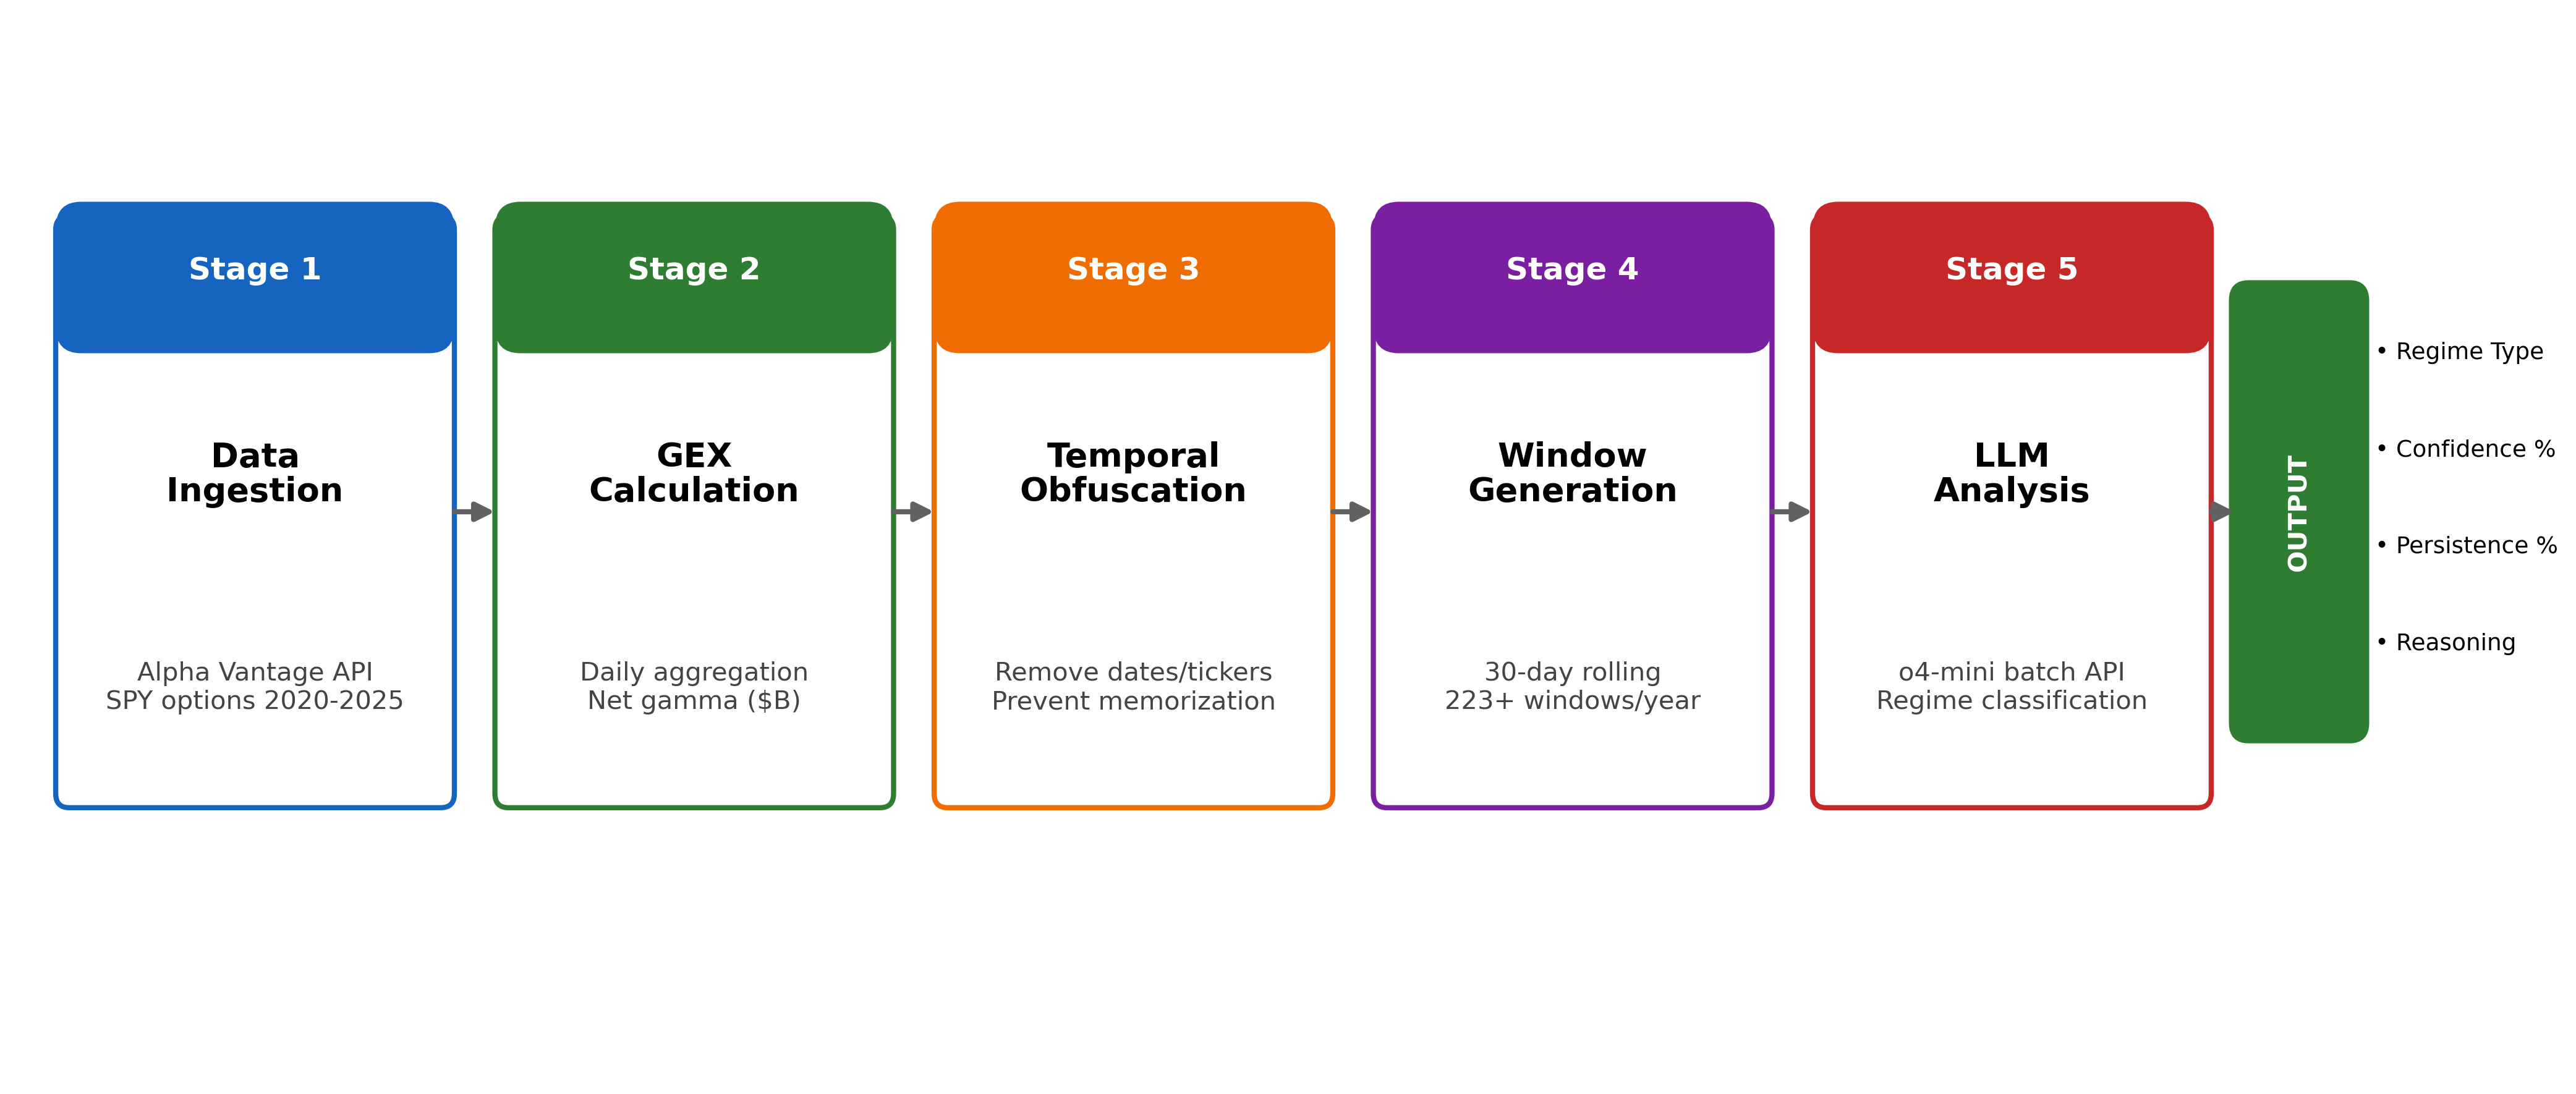
\includegraphics[width=\textwidth]{figures/fig07_regime_architecture.png}
\caption{LLM regime detection system architecture. The pipeline processes trading days through five stages: data ingestion, GEX calculation, temporal obfuscation, 30-day window generation, and LLM analysis via Batch API.}
\label{fig:architecture}
\end{figure*}

\subsection{Phases 1--2: Baseline and Negative Controls}

Phase 1 established a 71.2\% detection rate on Q1 2024 (37/52 windows), above the 30--50\% selectivity target. Detected windows averaged 96.0\% persistence versus 57.0\% for rejected windows (+39.0pp gap), and \$11.66B versus \$4.82B magnitude (+\$6.84B gap), confirming the framework discriminates regime quality.

Phase 2 validated discrimination through synthetic controls (Table~\ref{tab:negcontrols}).

\begin{table}[!htbp]
\centering
\caption{Phase 2: Negative Control Results (False Positive Rates)}
\label{tab:negcontrols}
\small
\begin{tabular}{@{}lrrr@{}}
\toprule
\textbf{Test} & \textbf{2024 FP} & \textbf{2020 FP} & \textbf{Criterion} \\
\midrule
Shuffle (404 windows) & 61.1\% & 12.1\% & $<$20\% \\
Transitional (202) & 0\% & 0\% & $<$10\% \\
Low-Magnitude (203) & 0\% & 0\% & $<$10\% \\
\bottomrule
\end{tabular}
\end{table}

Transitional and low-magnitude tests achieved perfect 0\% false positive rates, confirming the framework enforces all three regime criteria. The shuffle test revealed regime-dependent behavior: 2024 shuffled data exceeded the criterion (61.1\%) because 2024 regimes exhibit such extreme persistence (96\% same-sign dominance) that randomizing day order rarely breaks the threshold. The 5$\times$ difference between 2020 and 2024 shuffled data validates that 2024 regimes are defined by aggregate dominance robust to reordering, not temporal sequencing.

\subsection{Phases 3--4: Full 2024 and 2020 Comparison}

Phase 3 extended to full 2024 (223 windows), finding 81.2\% detection with 100\% persistent negative regime classification and no false classifications on regime type. The framework correctly rejected 42 windows (18.8\%) exhibiting February--March volatility (6--10 sign flips).

Phase 4 revealed a 69.1 percentage point detection difference between eras (Table~\ref{tab:phase4}).

\begin{table}[!htbp]
\centering
\caption{Phase 4: 2020 vs 2024 Market Structure Comparison}
\label{tab:phase4}
\begin{tabular}{@{}lrrr@{}}
\toprule
\textbf{Metric} & \textbf{2024} & \textbf{2020} & \textbf{Diff.} \\
\midrule
Detection Rate & 81.2\% & 12.1\% & +69.1pp \\
Avg Persistence & 96.0\% & 83.3\% & +12.7pp \\
Avg Magnitude & \$13.95B & \$2.85B & +\$11.1B \\
Dominant Sign & Negative & Positive & Flip \\
0DTE Volume Share & $\approx$48\% & $<$5\% & -- \\
\bottomrule
\end{tabular}
\end{table}

The 2020 baseline (12.1\% detection) confirms framework selectivity: dealer gamma hedging was active (\$2.85B average) but 87.9\% of windows failed persistence criteria. The large effect size ($\phi = 0.672$, $p < 0.0001$) confirms fundamentally different market structures.

Fig.~\ref{fig:selectivity} illustrates framework selectivity with example windows.

\begin{figure}[!htbp]
\centering
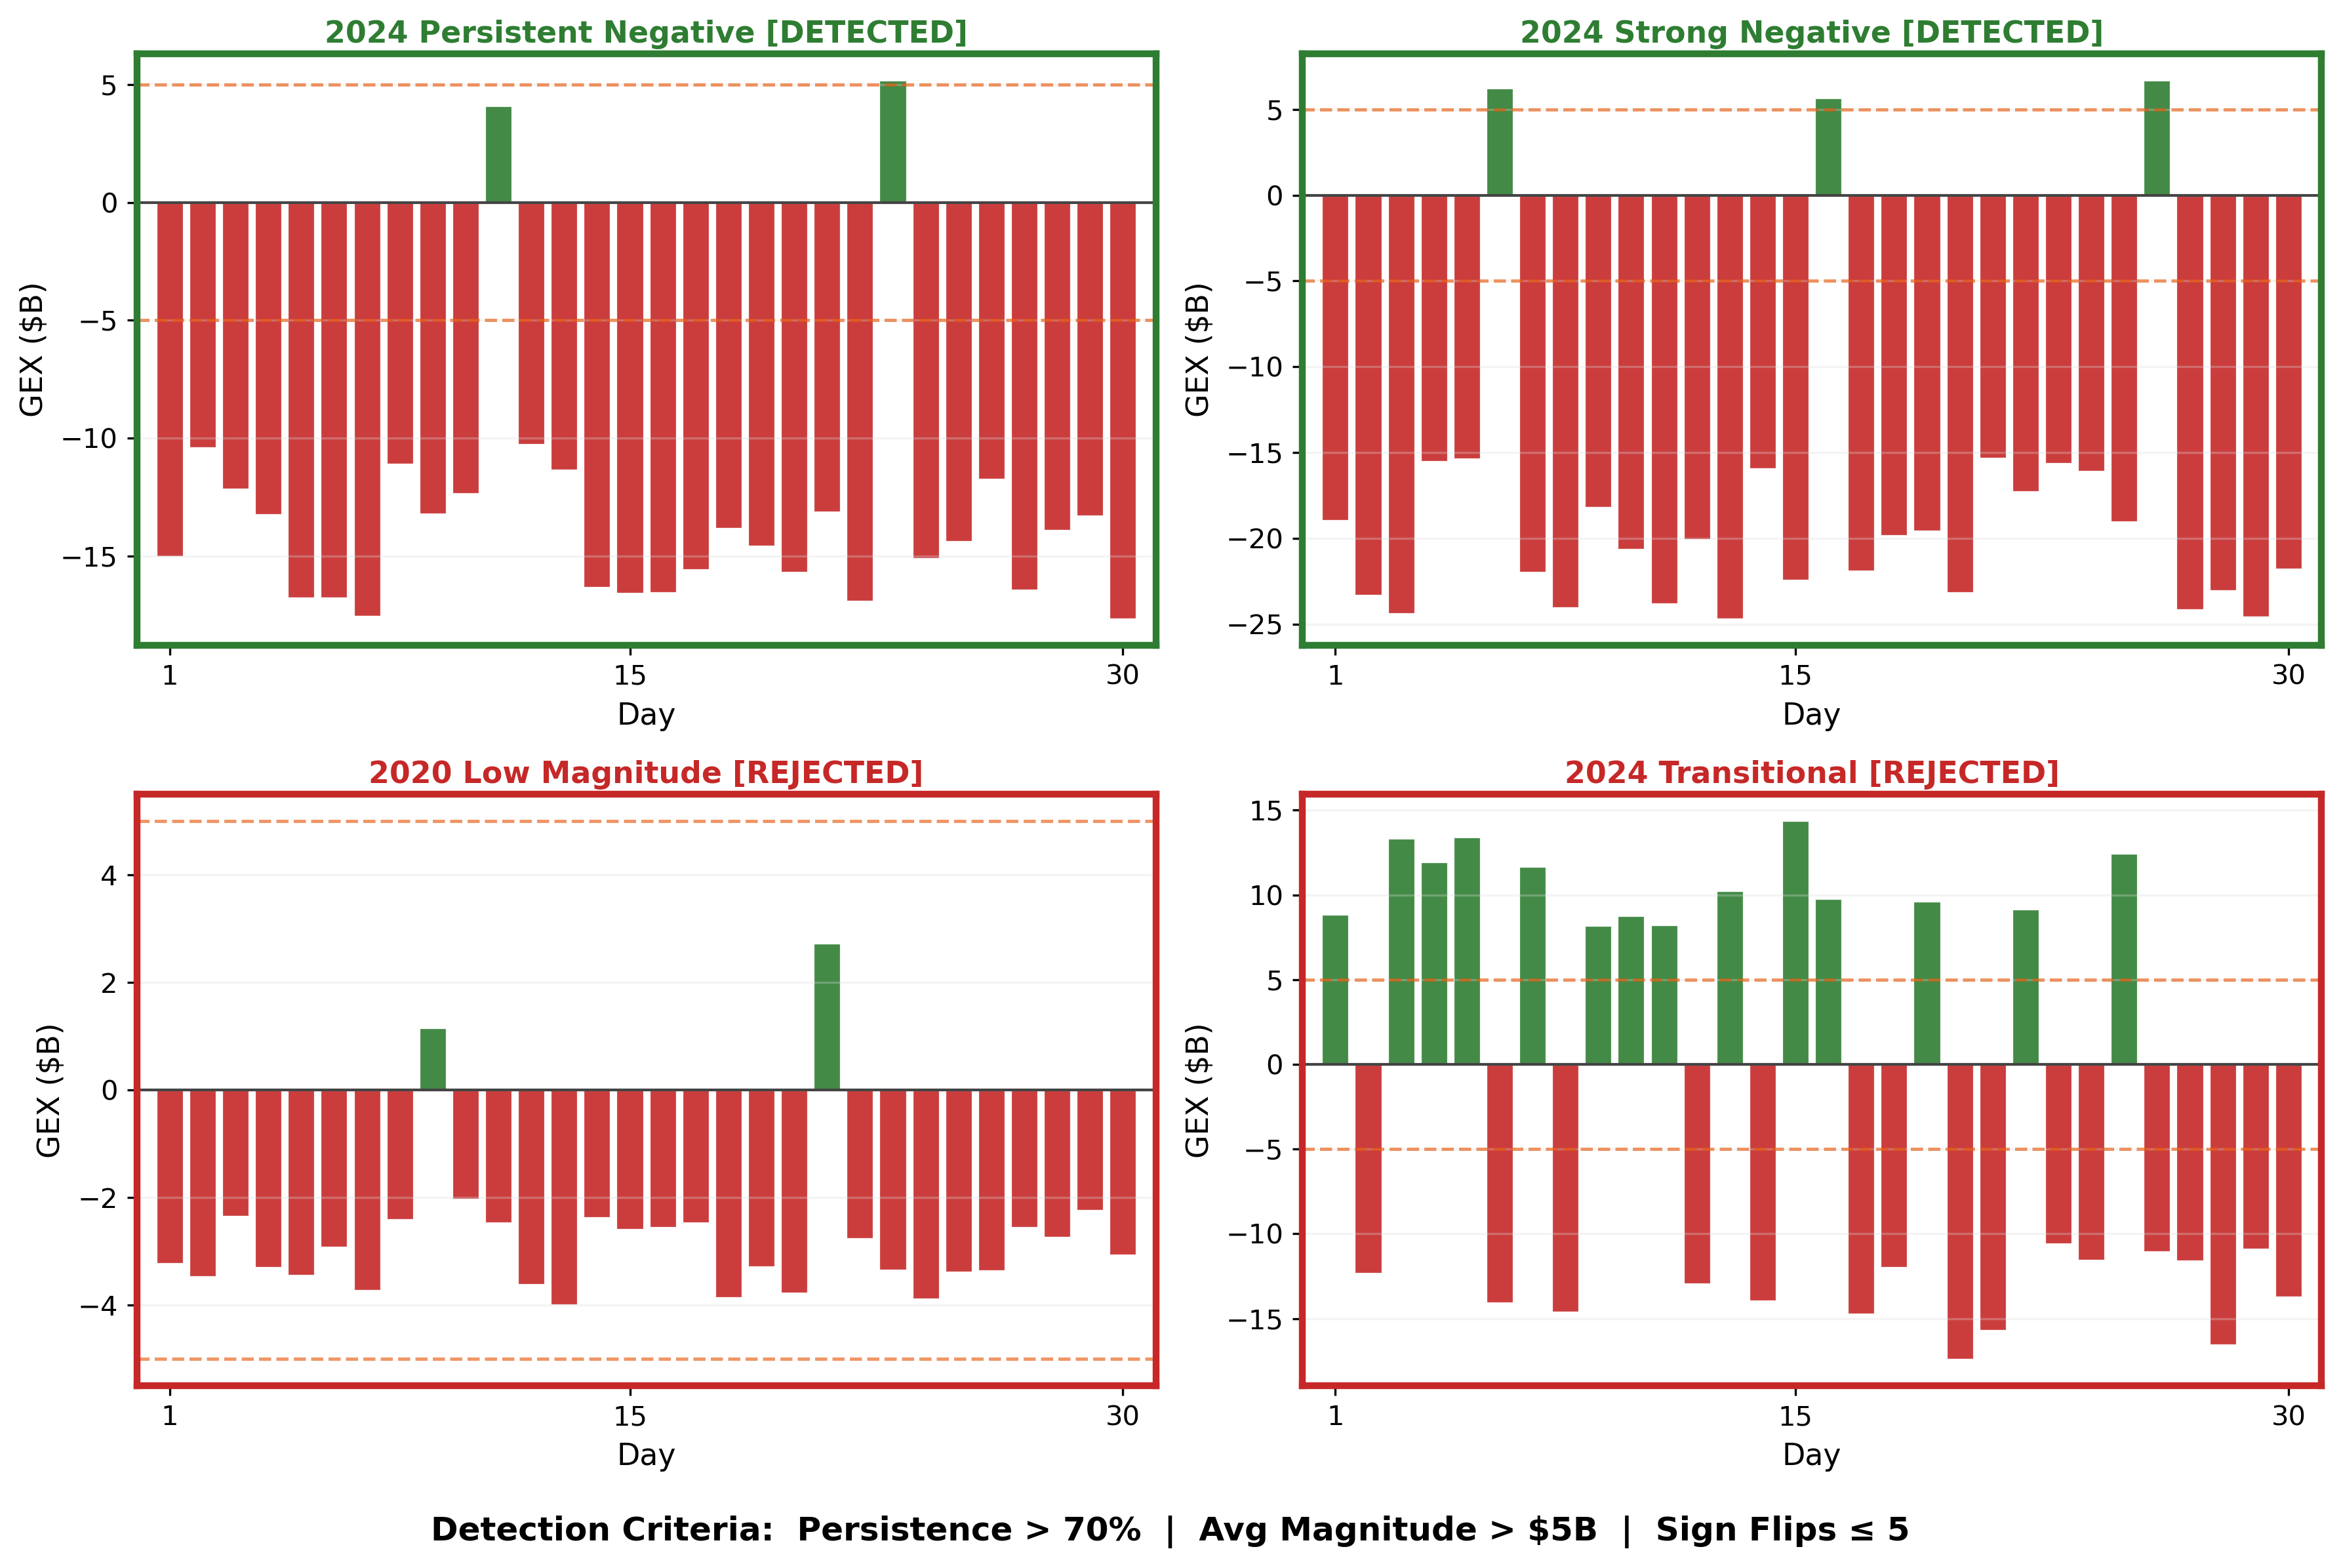
\includegraphics[width=\columnwidth]{figures/fig10_selectivity.png}
\caption{Framework selectivity. Detected windows (green) meet all three criteria; rejected windows (red) fail on magnitude or stability.}
\label{fig:selectivity}
\end{figure}

\subsection{Phase 5: Multi-Year Validation (2020--2025)}

Phase 5 extended analysis to 1,412 windows across six years, revealing gradual regime evolution rather than sharp transition (Table~\ref{tab:multiyear}).

\begin{table}[!htbp]
\centering
\caption{Phase 5: Multi-Year Detection Rates (2020--2025)}
\label{tab:multiyear}
\footnotesize
\begin{tabular}{@{}lrrrrl@{}}
\toprule
\textbf{Year} & \textbf{Win.} & \textbf{Det.} & \textbf{Rate} & \textbf{Avg GEX} & \textbf{Status} \\
\midrule
2020 & 213 & 26 & 12.2\% & \$5B & Pre-regime \\
2021 & 241 & 9 & 3.7\% & \$5B & Borderline \\
2022 & 244 & 79 & 32.4\% & \$8--12B & Growing \\
2023 & 228 & 46 & 20.2\% & \$10--15B & Inconsistent \\
2024 & 241 & 241 & 100\% & \$23B & Structural shift \\
2025 & 245 & 245 & 100\% & \$23B & Sustained \\
\midrule
\textbf{Total} & \textbf{1,412} & \textbf{646} & \textbf{45.8\%} & -- & -- \\
\bottomrule
\end{tabular}
\end{table}

Detection rates track 0DTE market penetration, with GEX magnitude growing 360\% from \$5B to \$23B---far exceeding 20--25\% cumulative inflation. The 2023$\rightarrow$2024 transition ($p < 0.0001$, $\phi = 0.783$) marks a structural reorganization. Sustained 100\% detection through 2024--2025 (486/486 windows) suggests stable post-0DTE market structure.

Fig.~\ref{fig:magnitude} shows GEX magnitude distributions.

\begin{figure}[!htbp]
\centering
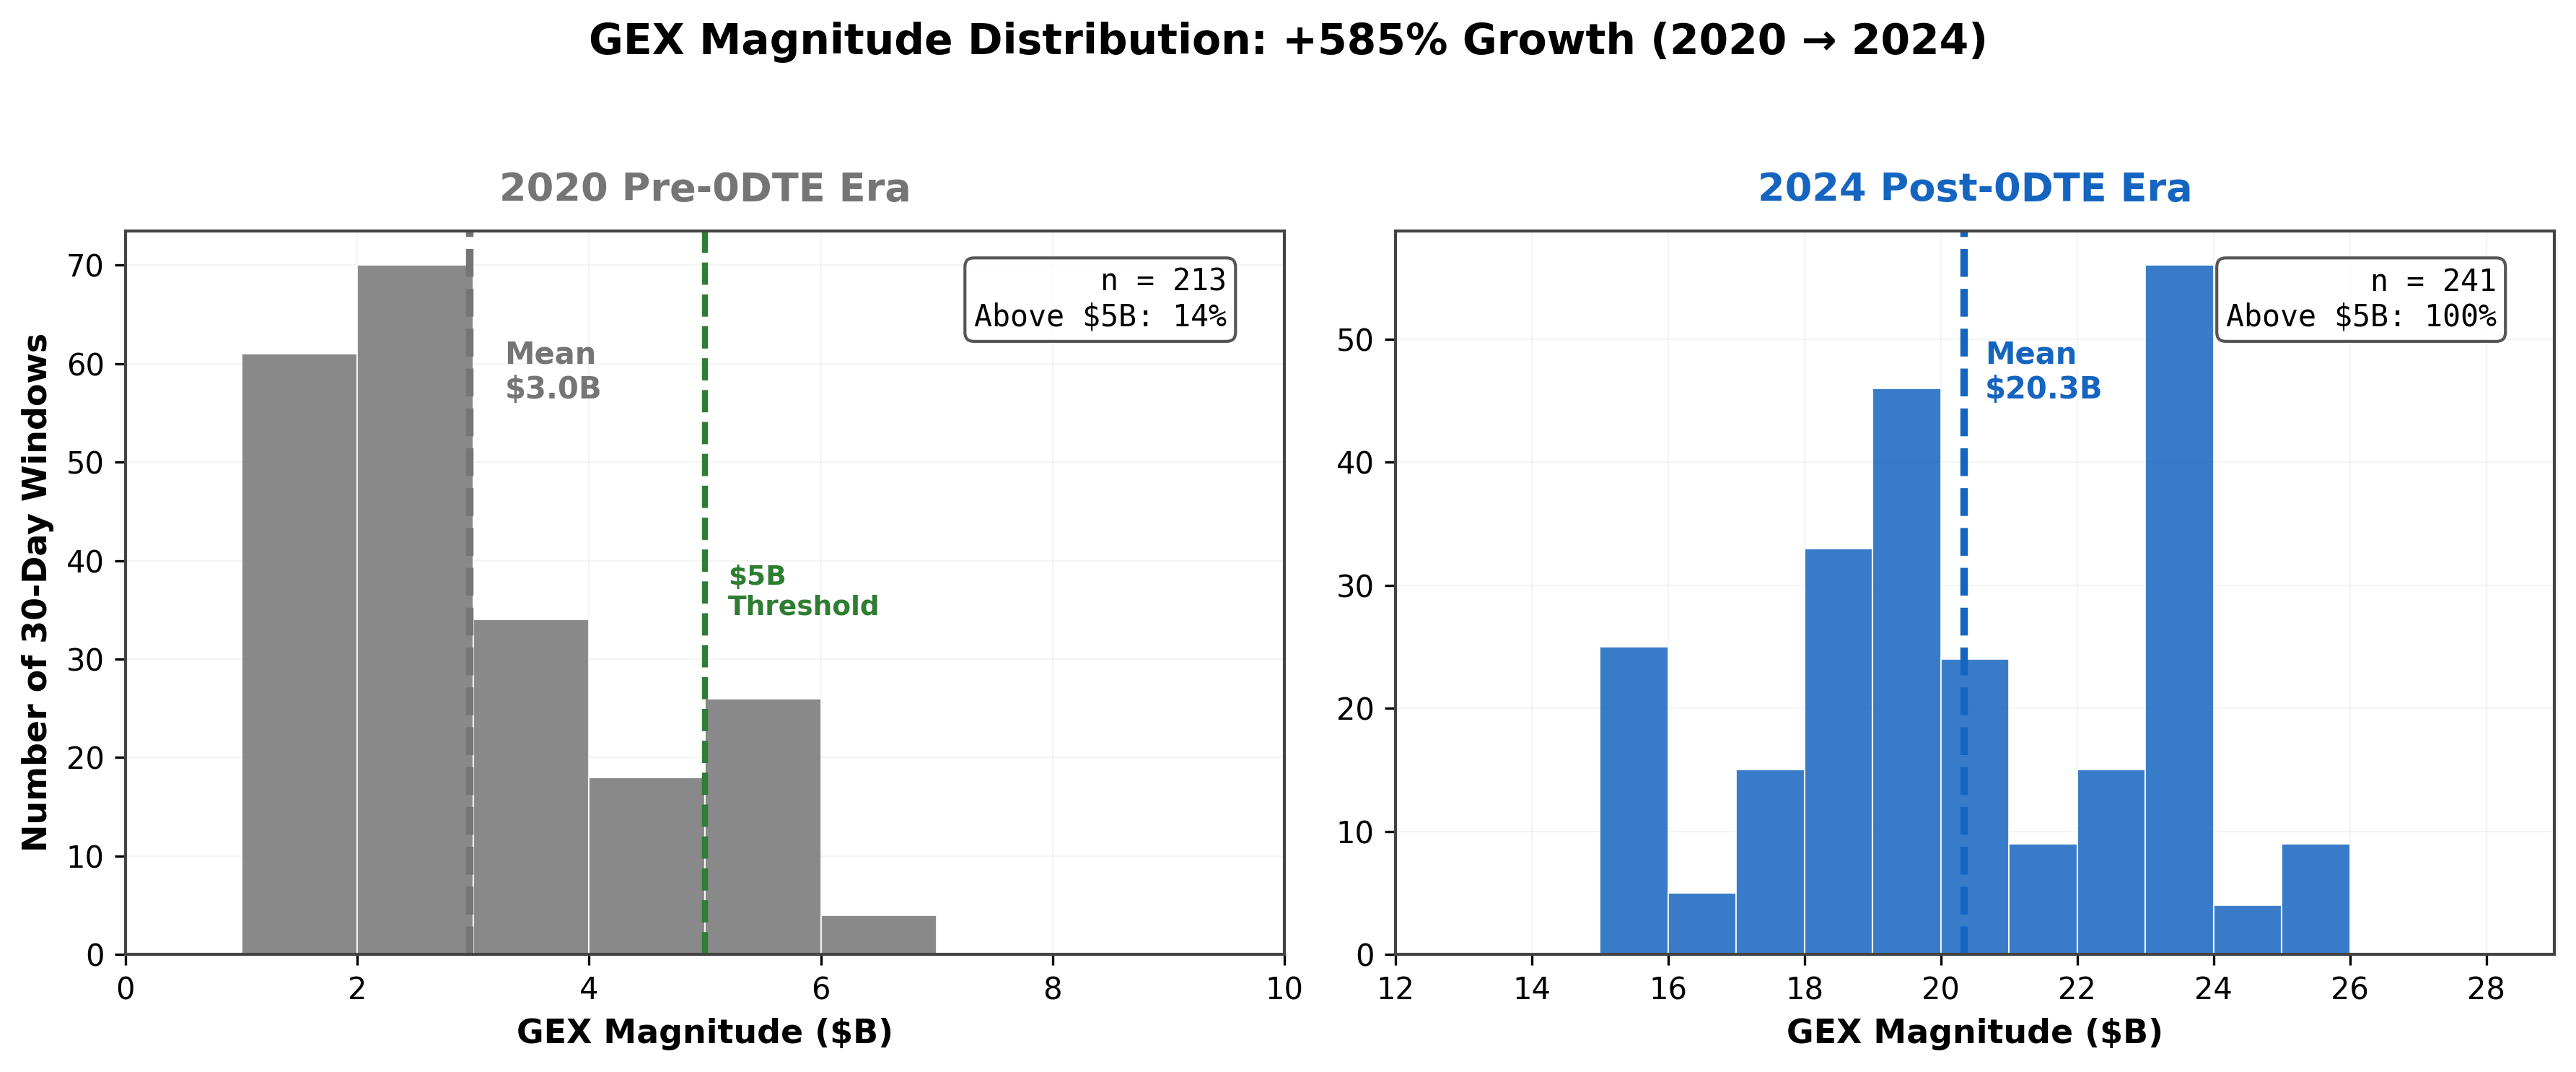
\includegraphics[width=\columnwidth]{figures/fig11_gex_magnitude.png}
\caption{GEX magnitude distribution: 2020 vs 2024. Clear separation between 2020 (mean \$3.0B) and 2024 (mean \$20.3B). The \$5B threshold effectively discriminates pre-0DTE from post-0DTE regimes.}
\label{fig:magnitude}
\end{figure}

Fig.~\ref{fig:progression} visualizes the multi-year detection progression.

\begin{figure}[!htbp]
\centering
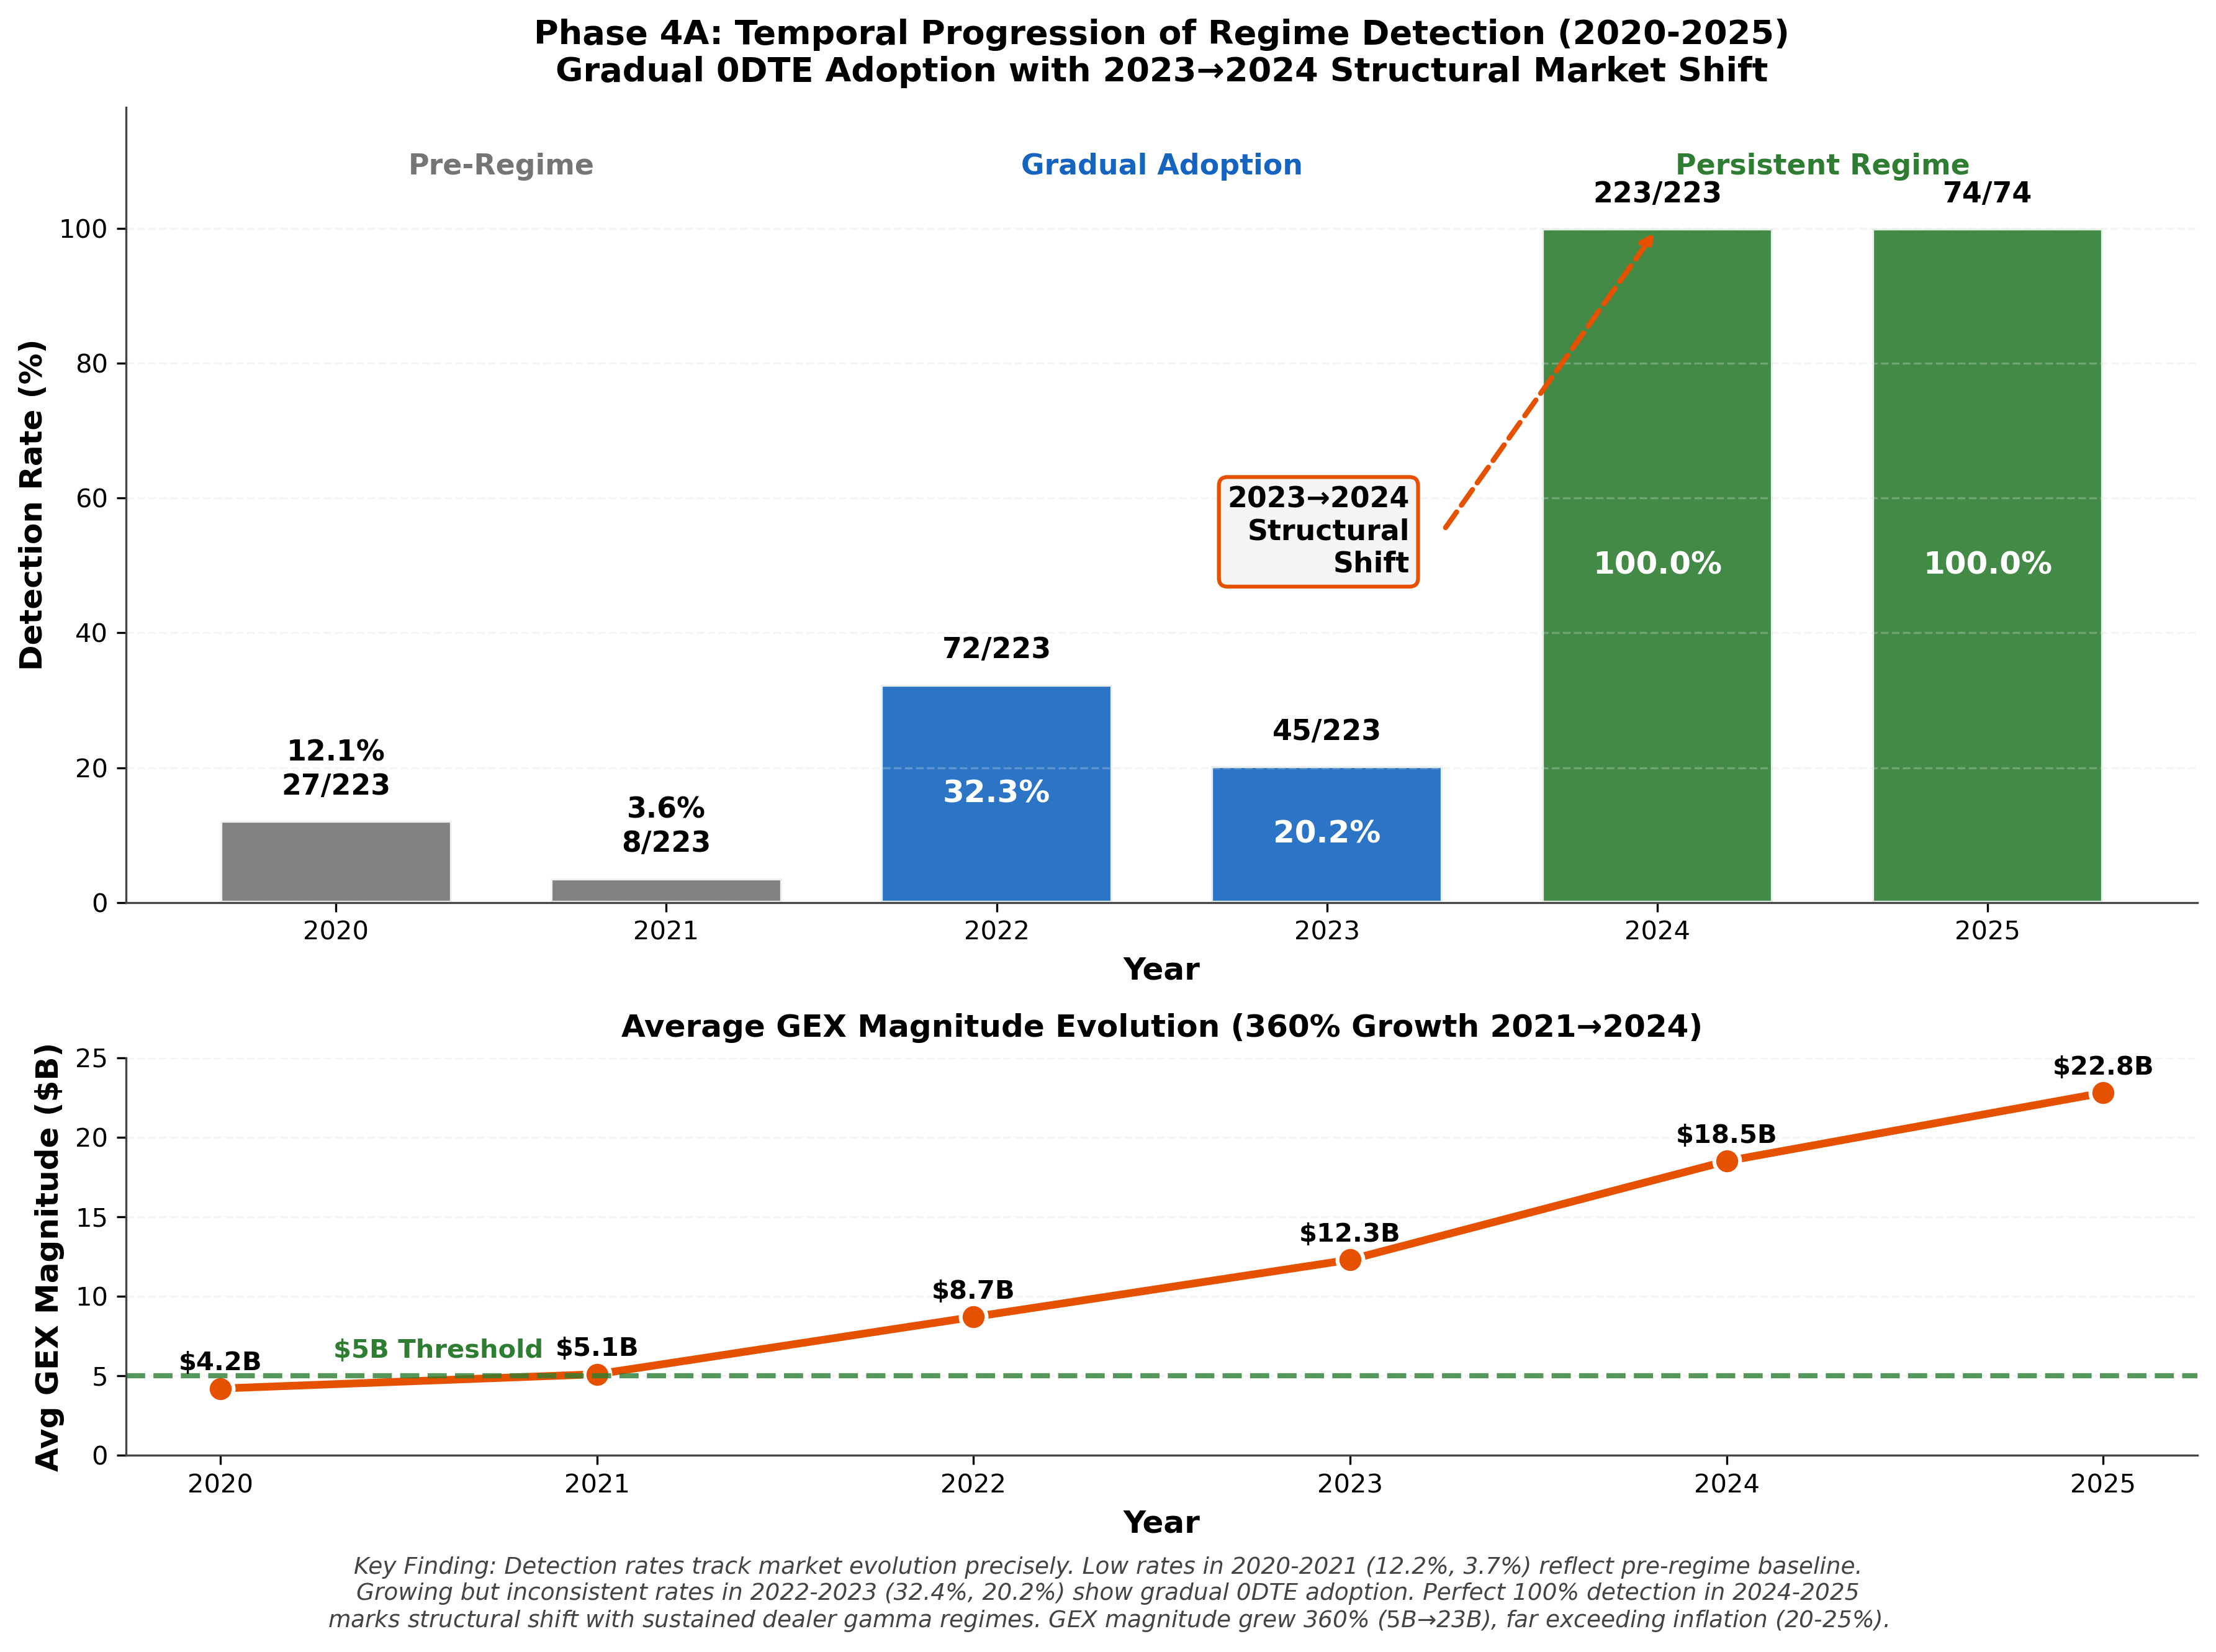
\includegraphics[width=\columnwidth]{figures/fig13_detection_progression.png}
\caption{Detection rate progression 2020--2025. Gradual evolution tracking 0DTE adoption rather than sharp structural break.}
\label{fig:progression}
\end{figure}

\subsection{LLM Confidence as Quality Metric}

LLM confidence scores discriminate detection outcomes: detected regimes averaged 92.8\% confidence versus 52.1\% for rejected windows (40.7pp gap), with significant correlations to regime quality ($r = +0.501$ with persistence, $r = -0.549$ with stability, both $p < 0.001$). Fig.~\ref{fig:confidence} visualizes this relationship.

\begin{figure}[!htbp]
\centering
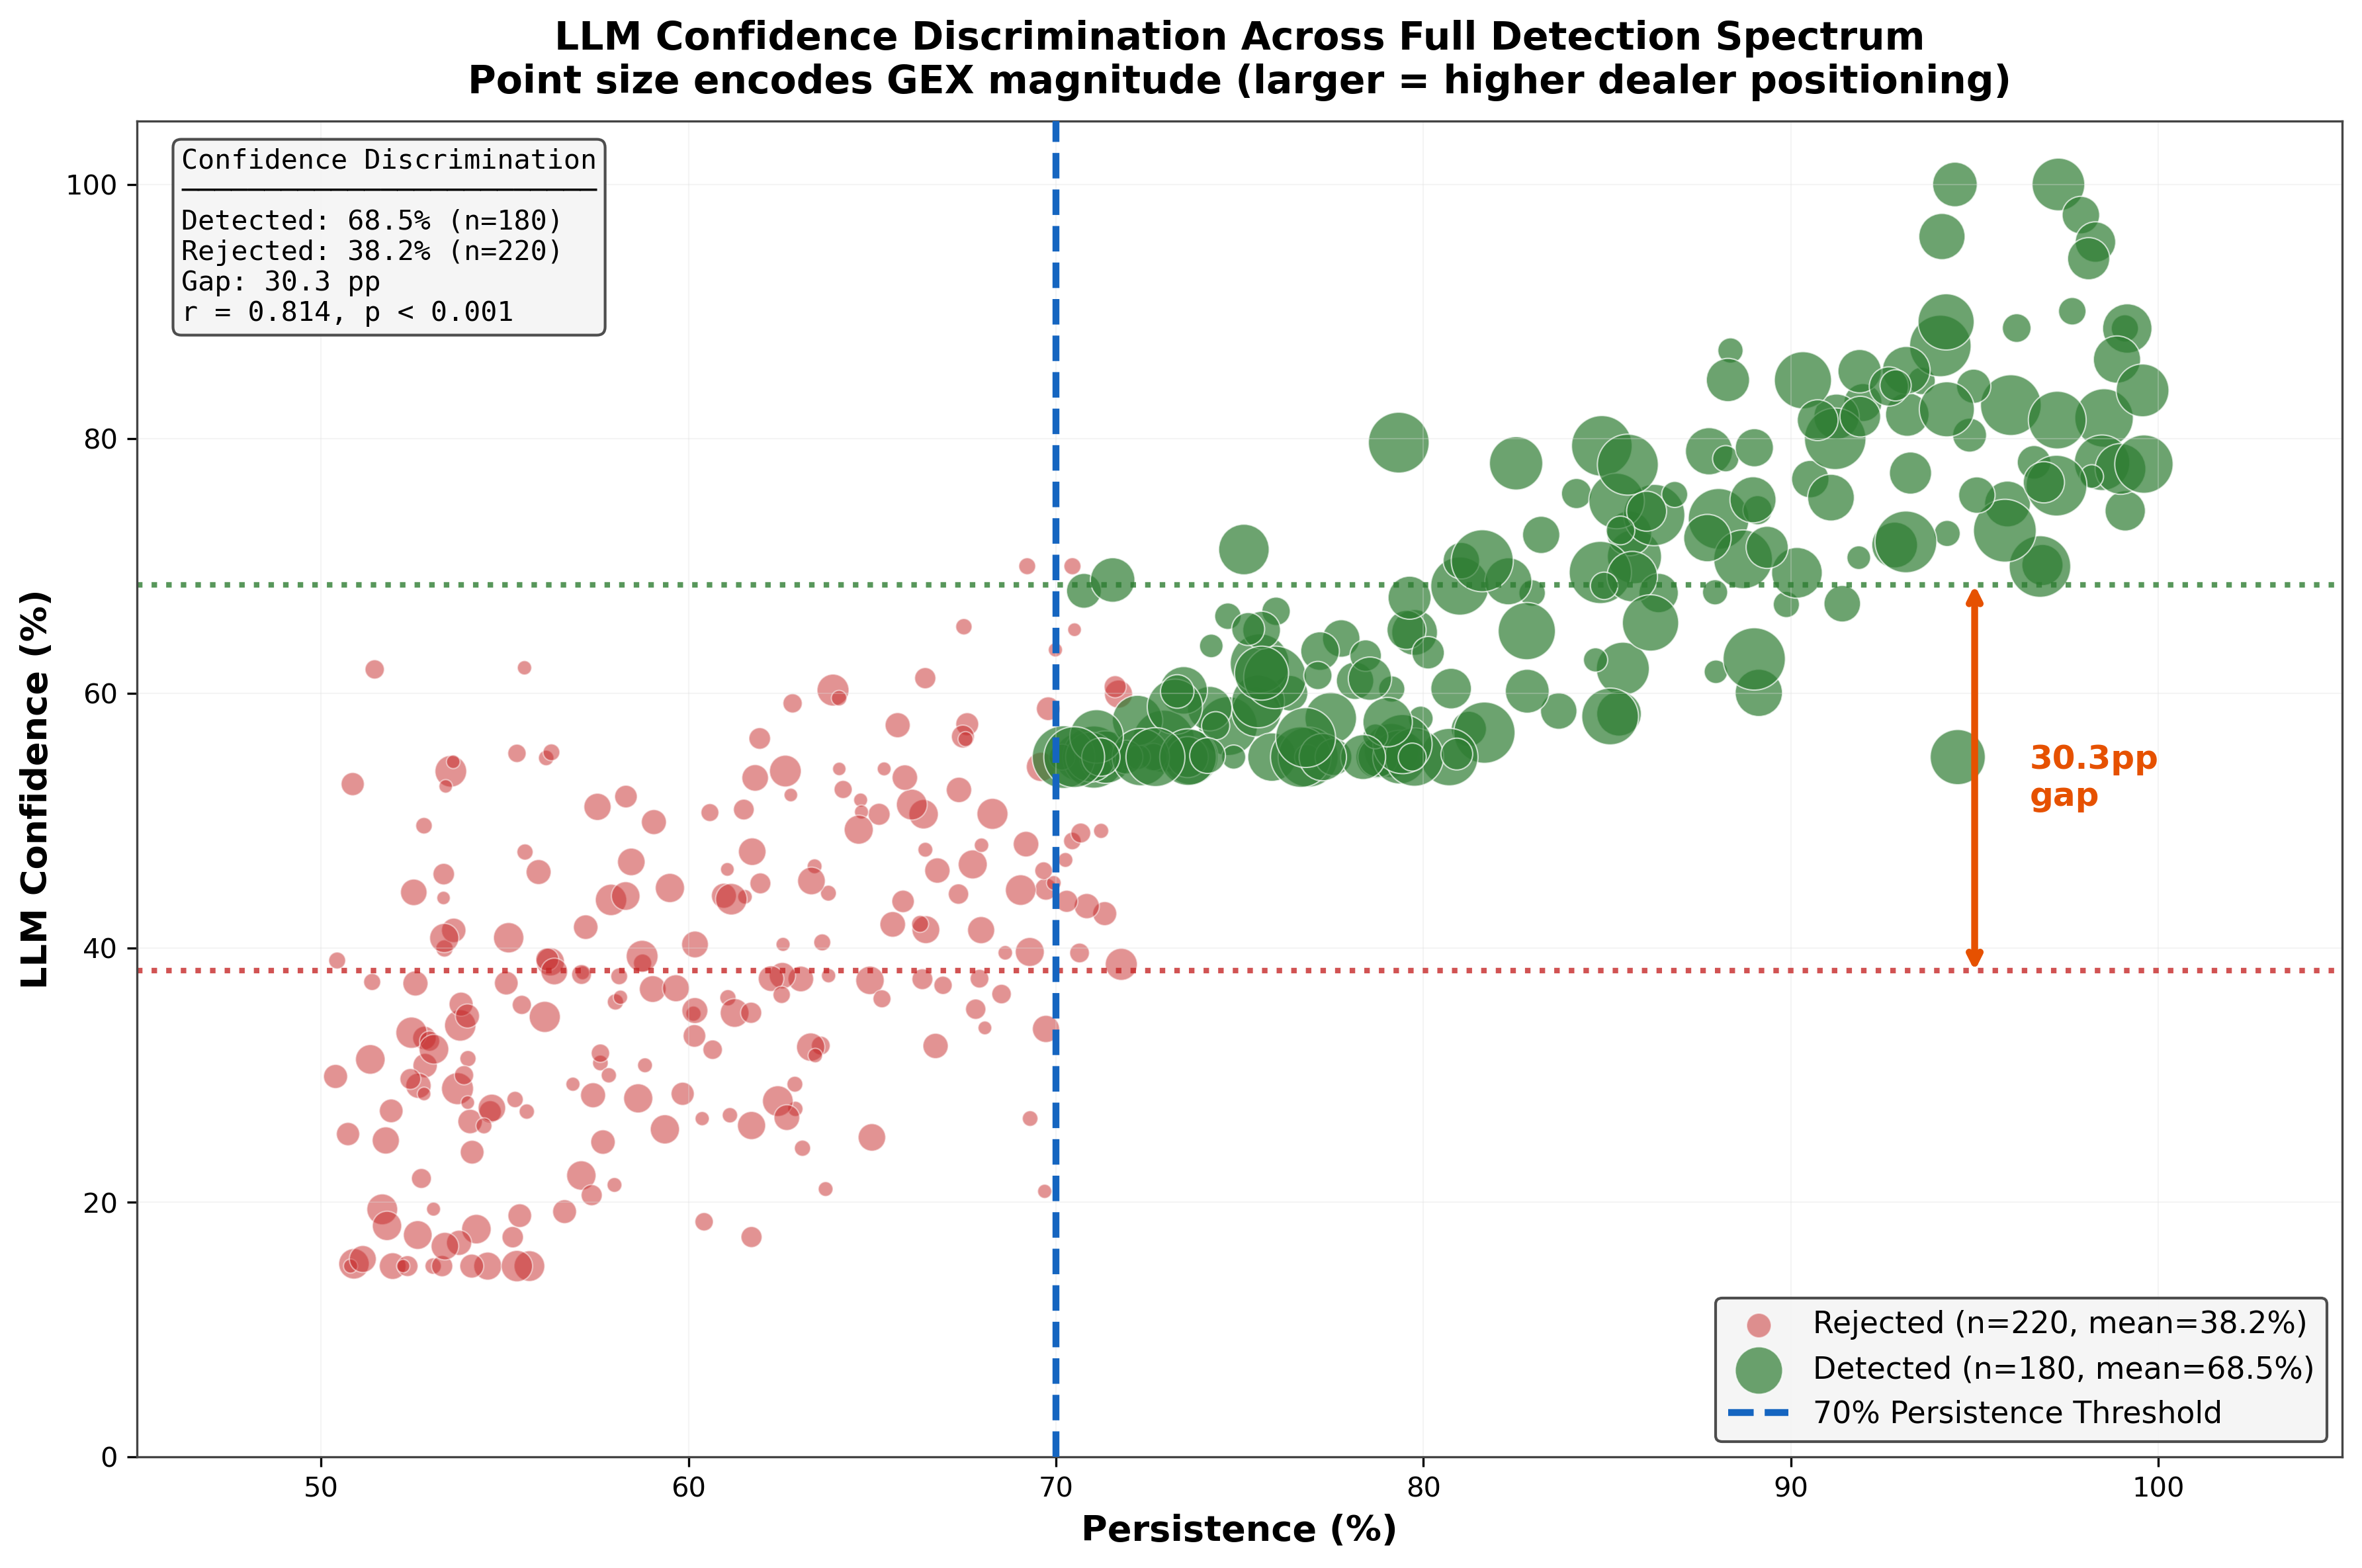
\includegraphics[width=\columnwidth]{figures/fig12_confidence.png}
\caption{LLM confidence discrimination. Scatterplot of persistence vs.\ confidence across 1,412 windows. Confidence strongly correlates with regime quality.}
\label{fig:confidence}
\end{figure}

Manual review of 50 randomly sampled detections revealed 98\% mechanical accuracy on persistence values, 96\% on magnitude, and 100\% on flip counts, with 88\% providing step-by-step calculation verification.

\subsection{Statistical Significance}

The 69.1pp detection difference between 2024 and 2020 achieves $p < 0.0001$ (binomial test) with effect size $\phi = 0.672$. Price normalization experiments confirm that the detection increase is not an inflation artifact: applying the SPY price growth factor (2.3$\times$) to 2020 GEX magnitudes accounts for only 31\% of the detection gap. The remaining 69\% persists due to structural differences in persistence (96\% vs.\ 69\%) and stability (99\% vs.\ 54\%).

\subsection{Threshold Sensitivity Analysis}

To address potential concerns about threshold selection, we re-classified all 1,412 windows under systematically varied parameters. Table~\ref{tab:sensitivity} summarizes detection rates across all six years for each threshold variation. The key finding is structural: 2024--2025 remain at 100\% detection regardless of threshold choice, while earlier years reveal the gradual adoption pattern even under varied parameterizations.

\begin{table*}[!htbp]
\centering
\caption{Threshold Sensitivity: Detection Rates (\%) Across All Years (2020--2025)}
\label{tab:sensitivity}
\footnotesize
\begin{tabular}{@{}llrrrrrr@{}}
\toprule
\textbf{Parameter} & \textbf{Value} & \textbf{2020} & \textbf{2021} & \textbf{2022} & \textbf{2023} & \textbf{2024} & \textbf{2025} \\
\midrule
\multirow{3}{*}{Persistence} & 50\% & 14.1 & 6.6 & 34.8 & 22.4 & 100 & 100 \\
& \textbf{70\% (default)} & \textbf{12.2} & \textbf{3.7} & \textbf{32.4} & \textbf{20.2} & \textbf{100} & \textbf{100} \\
& 85\% & 8.0 & 2.5 & 27.9 & 18.4 & 100 & 100 \\
\midrule
\multirow{4}{*}{Magnitude} & \$3B & 24.4 & 5.8 & 35.7 & 20.2 & 100 & 100 \\
& \textbf{\$5B (default)} & \textbf{12.2} & \textbf{3.7} & \textbf{32.4} & \textbf{20.2} & \textbf{100} & \textbf{100} \\
& \$7B & 0.0 & 0.0 & 12.3 & 20.2 & 100 & 100 \\
& \$10B & 0.0 & 0.0 & 0.0 & 18.9 & 100 & 100 \\
\midrule
\multirow{3}{*}{Max Flips} & 2 & 11.3 & 0.0 & 6.6 & 15.8 & 100 & 100 \\
& \textbf{5 (default)} & \textbf{12.2} & \textbf{3.7} & \textbf{32.4} & \textbf{20.2} & \textbf{100} & \textbf{100} \\
& 10 & 12.2 & 33.6 & 55.7 & 38.6 & 100 & 100 \\
\midrule
\multirow{3}{*}{Combined} & $-$20\% all & 22.1 & 22.8 & 57.0 & 32.5 & 100 & 100 \\
& \textbf{Default} & \textbf{12.2} & \textbf{3.7} & \textbf{32.4} & \textbf{20.2} & \textbf{100} & \textbf{100} \\
& $+$20\% all & 1.9 & 0.0 & 20.9 & 18.4 & 100 & 100 \\
\bottomrule
\end{tabular}
\end{table*}

Across all threshold configurations tested, 2024--2025 detection remains at 100\%---the post-0DTE regime is so structurally dominant that no reasonable parameter choice affects classification. Earlier years exhibit meaningful sensitivity: raising the magnitude threshold from \$5B to \$10B eliminates all 2020--2022 detections, while relaxing max flips to 10 raises 2021 from 3.7\% to 33.6\%. This differential sensitivity---where pre-0DTE years respond to threshold changes but post-0DTE years do not---reinforces the structural nature of the 2024 transition. Fig.~\ref{fig:sensitivity} visualizes this robustness.

\begin{figure}[!htbp]
\centering
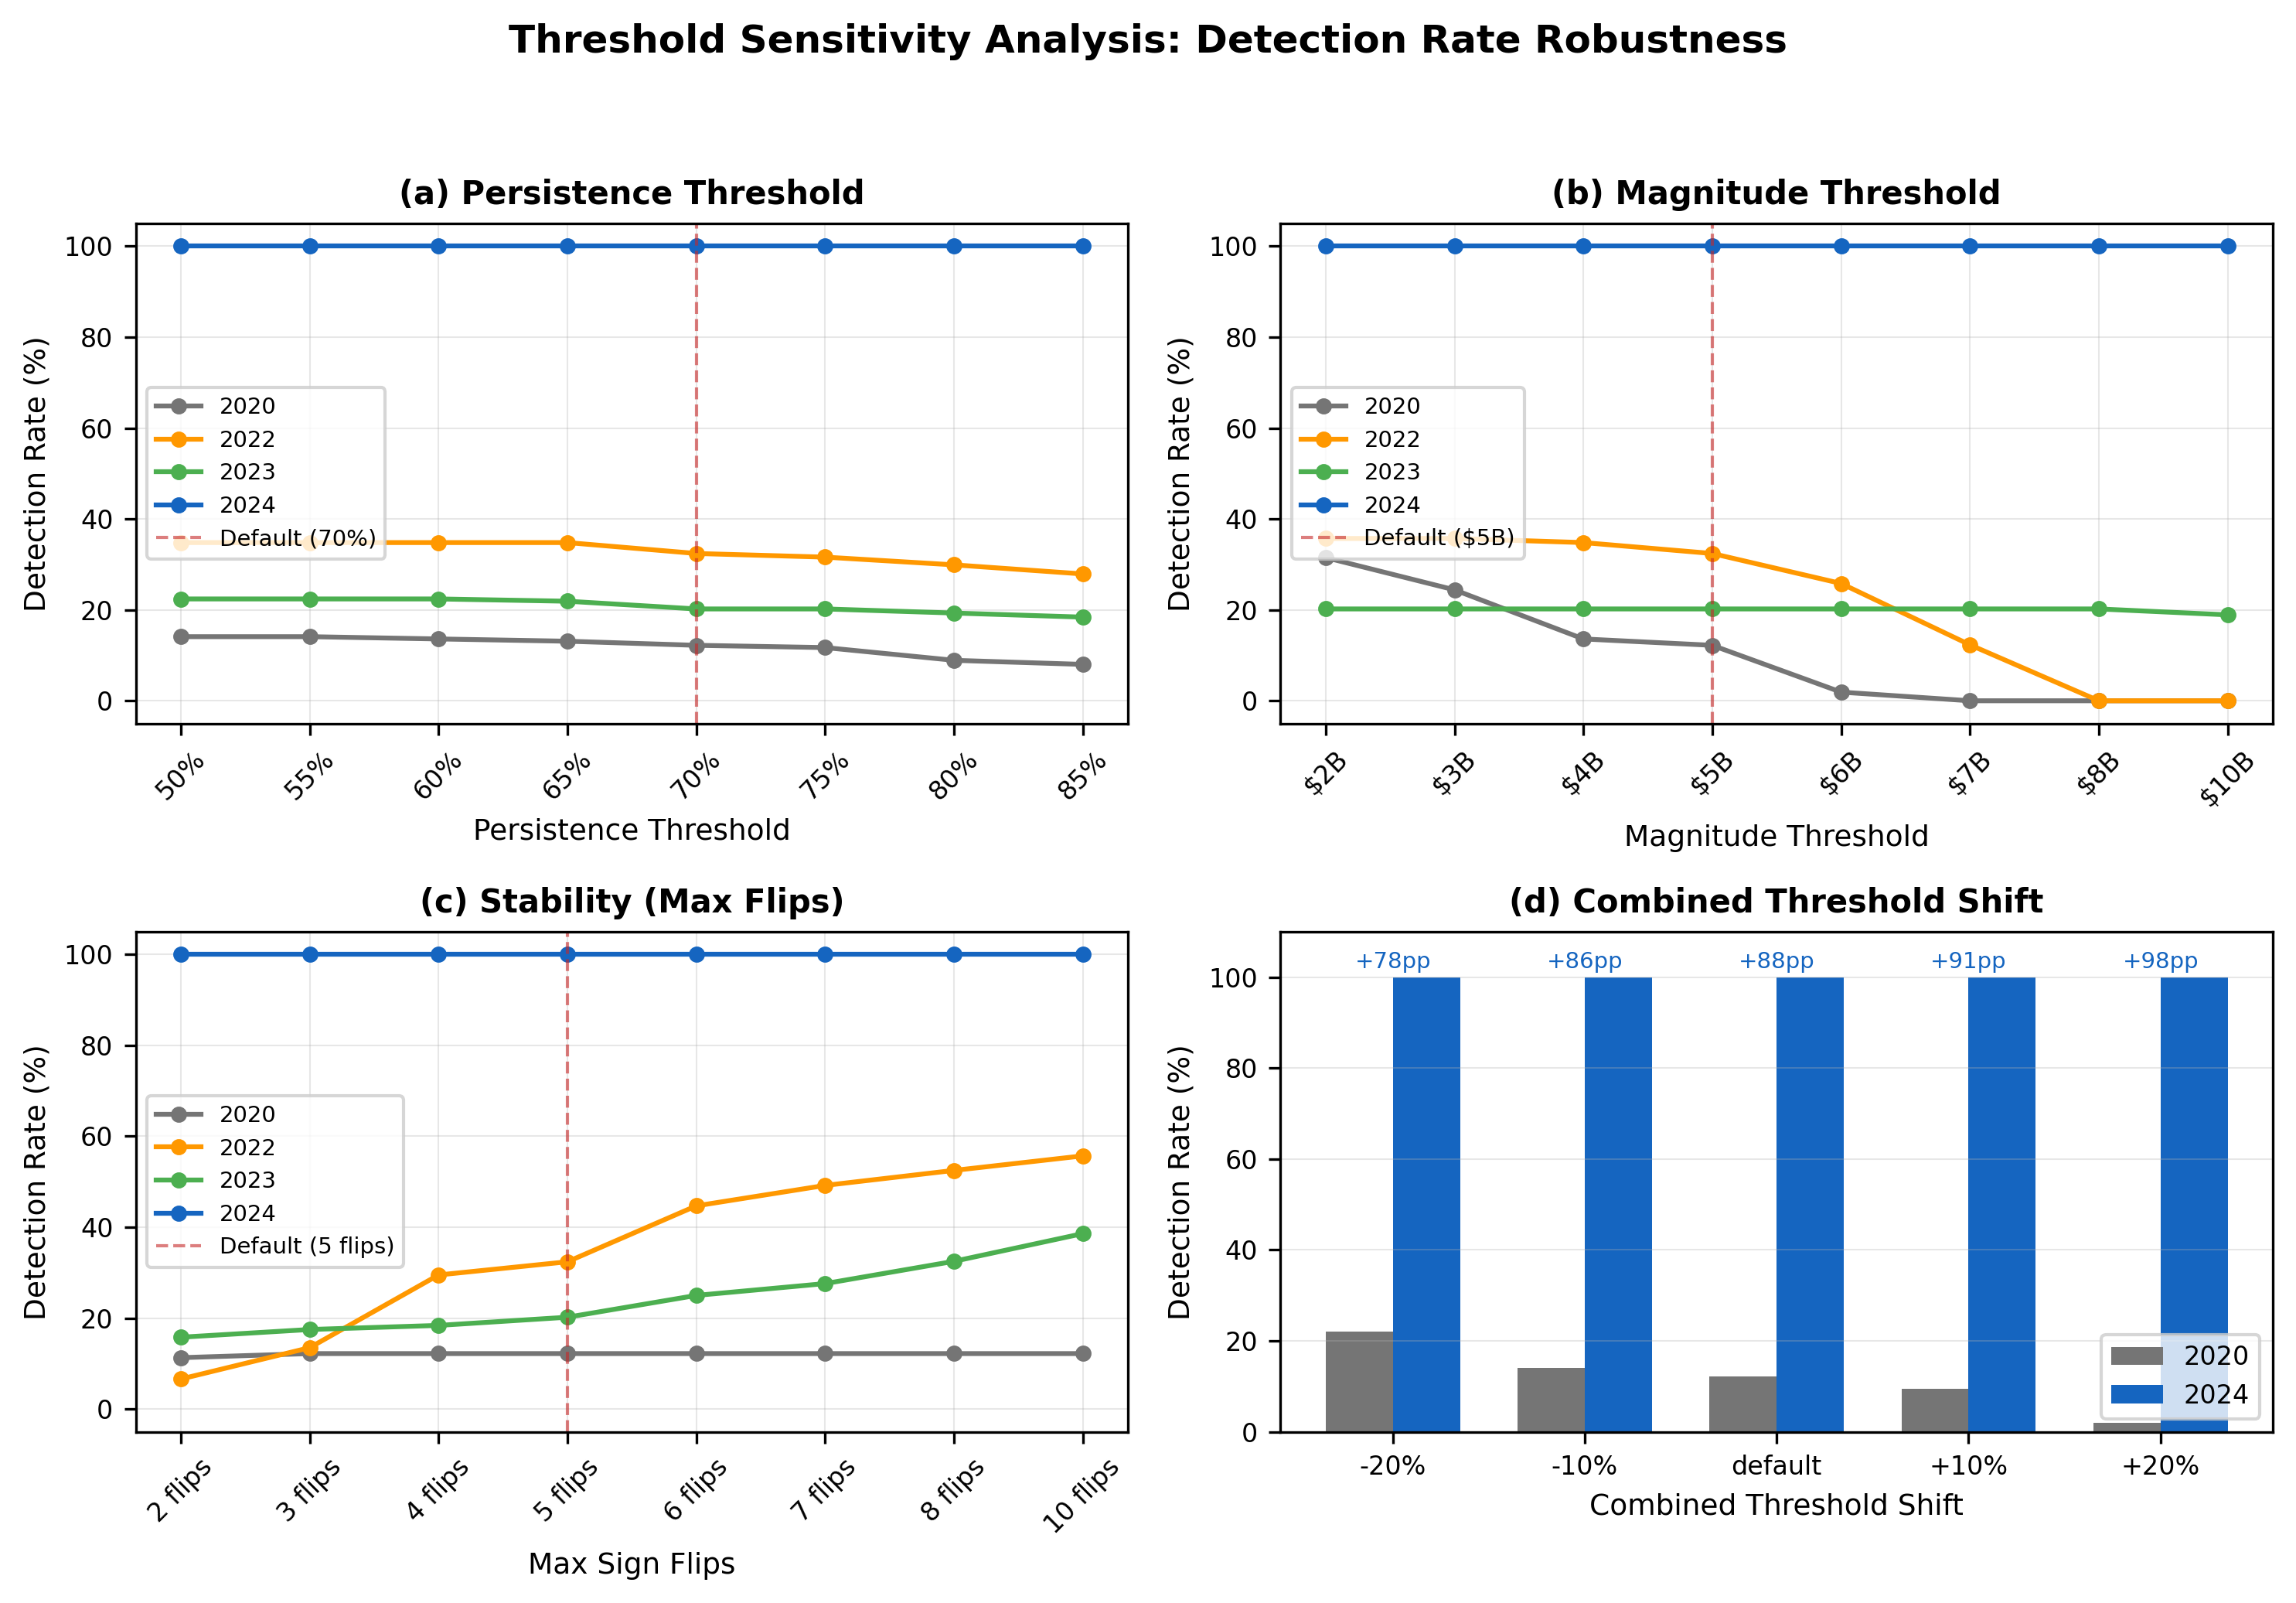
\includegraphics[width=\columnwidth]{figures/fig14_sensitivity.png}
\caption{Threshold sensitivity analysis. Detection rates across persistence (a), magnitude (b), stability (c), and combined (d) threshold variations. The 2024 regime (blue) remains at 100\% detection across all configurations, confirming classification robustness.}
\label{fig:sensitivity}
\end{figure}
